%%%%%%%%%%%%%%%%%%%%%%%%%%%%%%%%%%%%%
\section{Methods}
\label{sec:Methods}

A discussion of the steps necessary to implement the simulation of energy deposition in GEANT4 follows.
This involved writing the code for the simulation, as well as correctly interperting the output.
As such, this section is organzied by first examining the process of setting up the simulation and then will go into the analysis of the results from the toolkit.
\subsection{GEANT4 Implemenation}

A large focus of this work was on creating a working simulation of the GEANT4 toolkit.
Prelimary attemps were made to install GEANT4 on a windows based machine linking to Microscoft Visual Studio. While these attempts were sucessful, a larger scale computing enviroment was desired.
GEANT4 was then installed on the University of Tennessee's nuclear engineering computing cluster, along with the necessary visualation drivers and data files.
Brief documenation on compiling simple examples on the cluster are aviable at \texttt{necluster.engr.utk.edu/wiki/index.php/Geant4}\todo{Get URL to work}\footnote{It should be noted that this example uses the CMAKE build system (as per the GEANT4 recommendation) but a large majority of the examples still use GNUMake for building. This can be accomplished by adding \verb+source /opt/geant4/geant4-9.5p1/share/Geant4-9.5.1/geant4make/geant4make.sh+ to the user's \verb+.bashrc+.}. 
For convince a subversion repository was created to manage the developed code base, and all source code is available by anonymous checkout from \texttt{http://www.murphs-code-repository.googlecode.com/svn/trunk/layeredPolymerTracking}. Revision 360 was the code base used to generate the results shown in \ref{sec:Results}.
The following section provides implemenation specific details of the code base used to simulate the energy deposition in thin films.
It is organzied according to the three base classes that a user must implement in GEANT4, namely \verb+G4VUserDetectorConstruciton+, \verb+G4VUserPhysicsList+, and \verb+G4VuserPrimaryGeneratorAction+.
\subsubsection{Detector Geometry}

A detector geometry in GEANT4 is made up of a number of volumes.
The largest volume is the \verb+world+ volume which contains all other volumes in the detector geometry.
Each volume (an instance of \verb+G4VPhysicalVolume+) by assigning a position, a pointer to the mother volume and a pointer to its mother volume (or \verb+NULL+ if it is the \verb+world+ volume).
A volume's shape is described by \verb+G4VSolid+ which has a shape and the specific values for each dimension.
A volume's full properties is described by a logical volume.
A \verb+G4LogicalVolume+ includes a pointer to the geometrical properties of the volume (the solid) along with physical characteristics including:
\begin{itemize}
    \item the material of the volume,
    \item sensitive detectors of the volume and,
    \item any magnetic fields.
\end{itemize}
Listing \ref{lst:World} provides the implementation of the world physical volume.
The geometry was setup such that it is possible to define multiple layers of detectors, as shown in Figure \ref{fig:LayerDetectorGeo}.
%%%%%%%%%%%%%%%%%%%%%%%%% LISTING CODE %%%%%%%%%%%%%%%%%%%%%%%%%%
\lstinputlisting[linerange={217-220},caption=World Physical Volume,label=lst:World]{src/DetectorConstruction.cc}
The detector was described by creating creating a single layer of neutron absorber and gap material and placing it in another volume (the calorimeter).
The containing volume (calorimeter) was placed inside of the the physical world (Listing \ref{lst:Calo}).
%%%%%%%%%%%%%%%%%%%%%%%%% LISTING CODE %%%%%%%%%%%%%%%%%%%%%%%%%%
\lstinputlisting[linerange={226-229},caption=Calorimeter Volume,label=lst:Calo]{src/DetectorConstruction.cc}
The \verb+calorimeter+ was the mother volume for each layer. 
The code was developed such that the simulation of multiple layers can be easily set at compile time or by utilizing a run macro through the \verb+DetectorMessenger+ class.
Multiple repeated volume can be achieved in GEANT4 through \verb+G4PVReplica+ or \verb+G4PVParameterised+.
As each of the layers had the same geometry, \verb+G4PVReplica+ was chosen as the implementation (Listing \ref{lst:Layer}.
%%%%%%%%%%%%%%%%%%%%%%%%% LISTING CODE %%%%%%%%%%%%%%%%%%%%%%%%%%
\lstinputlisting[linerange={231-238},caption=Layer Volume,label=lst:Layer]{src/DetectorConstruction.cc}
Finally, the neutron absorber and gap material were defined as single cylinders which were then placed in the layer mother volume (Listing \ref{lst:GapAbs}).
The size of these solids (and the materials) could be set either at compile time through \verb+DetectorConstruction+ constructor or by using the \verb+DetectorMessenger+ in the run macro.
Figure \ref{fig:LayerDetectorGeo} shows a rendering of the 10 layers of the detector with the trajectories from a gamma event.
%%%%%%%%%%%%%%%%%%%%%%%%% LISTING CODE %%%%%%%%%%%%%%%%%%%%%%%%%%
\lstinputlisting[linerange={241-249},caption=Absorber and Gap Volumes,label=lst:GapAbs]{src/DetectorConstruction.cc}
\begin{figure}[h] 
    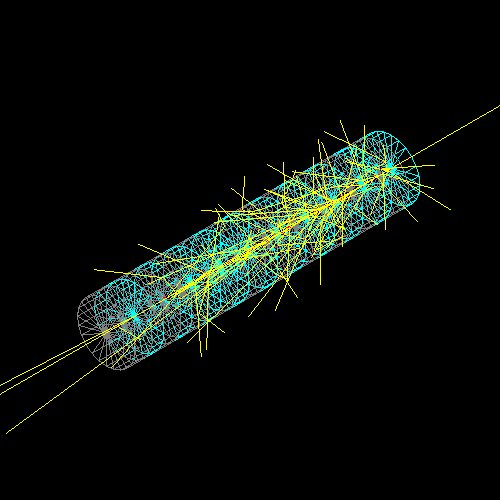
\includegraphics[width=\figurewidth]{10LayerGamma}
	\caption{10 Layer Detector with a simulated gamma event}
    \label{fig:LayerDetectorGeo}
\end{figure}

\subsubsection{Physics Lists}

The user of the GEANT4 toolkit is responsible for selecting the proper physics processes to model in the \verb+PhysicsList+.
This is unlike other transport codes (such as MCNPX) where basic physics are enabled by default and the user only has select the appropriate cards.
However, GEANT4 does provide examples of implemented \verb+PhysicsLists+ as wells as modular physics lists which provide a way to construct a physics list by combing physics list.
Thus, extensive use of \verb+G4ModularPhysicsList+ was employed to handle the assigning of the physics processes to each particle in the correct order.
The physics lists chosen for this simulation are listed below:
\begin{itemize}
    \item \verb+G4EmStandardPhysics+ The electromagnetic physics defines the electrons, muons, and taus along with their corresponding neutrinos. For electrons, the primary concern of this simulation, multiple scattering, electron ionization, and electron bremsstrahlung processes were assigned.  In addition the positron is defined and the multicle scattering process, electron ionization process, electron bremsstrahlung process and positiron annihilation is assigned \cite{cern_physics_2012}.
    \item \verb+G4EmLivermorePhysics+ The Livermore phyiscs process extend the \verb+EMStandardPhyiscs+ down to low (250 eV) energies. Even lower energies can be reached by including \verb+G4DNAPhysics+. These phyisics processes extended with \verb+G4EmLivermorePhysics+ are the photo-electoric effect, Compton scattering, Rayleight scattering, gamma conversion, Ionisation and Bremsstrahlung\cite{cern_physics_2012}. 
    \item \verb+HadronPhysicsQGSP_BERT_HP+ Hadronic physics are included to model the nuclear interactions. The chosen list is a Quark Gluon String Model for energies in the 5-25 GeV range, with a Bertini cascade model until 20 MeV.  Once a hadron has an energy of 20 MeV the high precision cross section driven models are applied\cite{cern_reference_2008}.
    \item \verb+G4IonPhysics+ Finally, to handle the transport of the charged ions resulting from an ${}^6\text{Li}(\text(n),\alpha){}^{3}\text{H}$ interaction the \verb+G4IonPhysics+ list was used.
\end{itemize}
%%%%%%%%%%%%%%%%%%%%%%%%% LISTING CODE %%%%%%%%%%%%%%%%%%%%%%%%%%
\lstinputlisting[linerange={10-25},caption=Implemented Physics List,label=lst:PhysicsListCtr]{src/PhysicsList.cc}
Finally, the default cut range was decreased from 1 cm to 1 nm in \verb+SetCuts()+ (Listing \ref{lst:PhyisicsListSetCuts}) 
%%%%%%%%%%%%%%%%%%%%%%%%% LISTING CODE %%%%%%%%%%%%%%%%%%%%%%%%%%
\lstinputlisting[linerange={36-48},caption=Implemented Physics List,label=lst:PhysicsListSetCuts]{src/PhysicsList.cc}
\subsubsection{Primary Event Generator}

The user is responsible for telling the simulation toolkit the primary event to generate.
While there is great flexibility to generate any source distribution, a particle gun was chosen for simplicity.
\verb+G4ParticleGun+ generates primary particle(s) with a given momentrum and position without any randomization.
The implementation of this is shown in Listing ~\ref{lst:PrimaryGeneratorAction}.
%%%%%%%%%%%%%%%%%%%%%%%%% LISTING CODE %%%%%%%%%%%%%%%%%%%%%%%%%%
\lstinputlisting[linerange={14-24},caption=Primary Event Generator,label=lst:PrimaryGeneratorAction]{src/PrimaryGeneratorAction.cc}
Actual primary particles are generated with \verb+GeneratePrimaries+, which uses the \verb+G4ParticleGun+ to determine the vertex of the primary event.
%%%%%%%%%%%%%%%%%%%%%%%%% LISTING CODE %%%%%%%%%%%%%%%%%%%%%%%%%%
\lstinputlisting[linerange={33-56},caption=Generate Primaries,label=lst:GeneratePrimaries]{src/PrimaryGeneratorAction.cc}

\subsection{Sensitive Detectors}

GEANT4 offers a myriad of differnet ways to output the results of a simulation.
It is possible to write out every track with the \verb+Verbose = 1+ option, create \verb+MultiFunctionalDetector+ and \verb+G4VPrimitiveScorer+, or implement a hit and readout based approach \cite{cern_detector_2012}.
Previous GEANT4 experience included \verb+G4VHit+ and \verb+G4VSensitiveDetector+ so this approach was used in this simulation. 
A hit is defined to be a snapshot of the physical inteaction of a track in a senstive region of a detector.
As the user is responsible for writing implementing \verb+G4VHit+ the hit can contain any information about the step, including
\begin{itemize}
	\item the postion and time of the step,
	\item the momentun and energy of the track,
	\item the energy deposition of the step,
	\item or information about the geometry.
\end{itemize}
For this simulation any information about the particle that could be recorded was recorded. 
This included the energy deposition, postion of the hit, momentrum, kineitic energy, track ID, parent ID, particle defination, volume and copy number (Listing \ref{lst:CaloHit}).
%%%%%%%%%%%%%%%%%%%%%%%%% LISTING CODE %%%%%%%%%%%%%%%%%%%%%%%%%%
\lstinputlisting[linerange={11-44,69-82},caption=Calorimeter Hit,label=lst:CaloHit]{include/CaloHit.hh}
The \verb+G4VSensitiveDetector+ is attached to a logical volume and is responsible for filling the hit collection.
This is accomplished in the \verb+ProcessHits+ of \verb+CaloSensitiveDetector+ (Listing \ref{lst:SD}).
%%%%%%%%%%%%%%%%%%%%%%%%% LISTING CODE %%%%%%%%%%%%%%%%%%%%%%%%%%
\lstinputlisting[linerange={29-61},caption=Sensitive Detector,label=lst:SD]{include/CaloSensitiveDetector.hh}
The simulation was designed so that a seperate sensitive detector was assigned to the gap and absorber.
While this is not stricly necessary as the geometric position determines what layer of the gap or absorber the hit occured in this made the analysis code easier to write.
A seperate method was written in \verb+DetectorConstruction+ to create the sensitive detectors and assign them to the proper logical volumes (Listing \ref{lst:SDAssign})
\verb+SetSensitiveDetectors()+ is called from the the constructor of \verb+DetectorConstruction+.
%%%%%%%%%%%%%%%%%%%%%%%%% LISTING CODE %%%%%%%%%%%%%%%%%%%%%%%%%%
\lstinputlisting[linerange={257-271},caption=Creating Sensitive Detectors,label=lst:SDAssign]{src/DetectorConstruction.cc}

\subsection{Analysis}

Analysis of hit collection was preformed with ROOT.  Once again there are other options (notably OpenScientist) but previous experiance was why ROOT was selected as the base for the Analysis framework.
A singleton class was written for the analysis which procssed the hit collections, assigning the various results to root histograms.
User action classes \verb+EventAction+ and \verb+RunAction+ are called at the begining and end of each run and event, respectively (Listing \ref{lst:EventAction},\ref{lst:RunAction}).
These clases allowed for the analysis code to be indepenet of the simulation.
%%%%%%%%%%%%%%%%%%%%%%%%% LISTING CODE %%%%%%%%%%%%%%%%%%%%%%%%%%
\lstinputlisting[linerange={11-37},caption=Event Action,label=lst:EventAction]{src/EventAction.cc}
%%%%%%%%%%%%%%%%%%%%%%%%% LISTING CODE %%%%%%%%%%%%%%%%%%%%%%%%%%
\lstinputlisting[linerange={16-25},caption=Run Action,label=lst:RunAction]{src/RunAction.cc}

\subsection{Determination of Energy Deposition}

The energy deposition of an event is calculated by the sum of all of the energy deposited by individual hits in the sensitive detector (Equation \ref{eq:EDepEvent}).
While it is possible to break down the energy deposition by which physics process caused the deposition, this was not implemented in order to avoid over complication.
\begin{equation}[h]
\label{eq:EDepEvent}
E_{\text{dep},\text{event}} = \sum{E_{\text{dep},\text{hit}} }
\end{equation}
\verb+ProcessHitCollection+ is called at the end of each event (Listing \ref{lst:PHC}).
Each hit is accesed and the layer at which it occurs is determined\footnote{C arrays start at 0, so memory is allocated for one more than the total number of layers. This allows for \verb|NUMLAYERS+1| to be used an index into the histogram for the total of all layers in the material (either \verb+gap+ or \verb+absorber+). }.
In addition the name of the volume is determined, and the energy depositon of the hit is added to the energy depostion of the event.
If the hit occured in the \verb+absorber+ layer and the particle is an electron the kinetic energy of that hit is also recorded.
%%%%%%%%%%%%%%%%%%%%%%%%% LISTING CODE %%%%%%%%%%%%%%%%%%%%%%%%%%
\lstinputlisting[linerange={121-175},caption=Process Hit Collection,label=lst:PHC]{src/Analysis.cc}

Finally, a run macro was written to control the entire run (Listing \ref{lst:RunMacro}).
The material and thickness of the detector are declared (made possible by the use of \verb+DetectorMessenger+), and then the detector is dynamically updated.
A \iso{Co}{60} source is simulated by shooting photons of the 1.1732 MeV and 1.3325 MeV.
The source particle is then changed to a neturon, and thermal (0.025 eV) neutrons are shot at the detector. 
The thickness of the absorber is then increased, the geometry updated, and the entire process repeated.
As these runs tend to take a large amount of time, GEANT4 was parallized for use with MPI to take advantage of the cluster computing power.
%%%%%%%%%%%%%%%%%%%%%%%%% LISTING CODE %%%%%%%%%%%%%%%%%%%%%%%%%%
\lstinputlisting[language=bash,linerange={1-25},caption=Run Macro,label=lst:RunMacro]{run1.mac}
